\documentclass[
  bibliography=totoc,     % Literatur im Inhaltsverzeichnis
  captions=tableheading,  % Tabellenüberschriften
  titlepage=firstiscover, % Titelseite ist Deckblatt
]{scrartcl}

% Paket float verbessern
\usepackage{scrhack}

% Warnung, falls nochmal kompiliert werden muss
\usepackage[aux]{rerunfilecheck}

% unverzichtbare Mathe-Befehle
\usepackage{amsmath}
% viele Mathe-Symbole
\usepackage{amssymb}
% Erweiterungen für amsmath
\usepackage{mathtools}
% Stromkreise zeichnen
\usepackage{tikz}
\usepackage[european]{circuitikz}

% Fonteinstellungen
\usepackage{fontspec}
% Latin Modern Fonts werden automatisch geladen
% Alternativ zum Beispiel:
%\setromanfont{Libertinus Serif}
%\setsansfont{Libertinus Sans}
%\setmonofont{Libertinus Mono}

% Wenn man andere Schriftarten gesetzt hat,
% sollte man das Seiten-Layout neu berechnen lassen
\recalctypearea{}

% deutsche Spracheinstellungen
\usepackage{polyglossia}
\setmainlanguage{german}


\usepackage[
  math-style=ISO,    % ┐
  bold-style=ISO,    % │
  sans-style=italic, % │ ISO-Standard folgen
  nabla=upright,     % │
  partial=upright,   % ┘
  warnings-off={           % ┐
    mathtools-colon,       % │ unnötige Warnungen ausschalten
    mathtools-overbracket, % │
  },                       % ┘
]{unicode-math}

% traditionelle Fonts für Mathematik
\setmathfont{Latin Modern Math}
% Alternativ zum Beispiel:
%\setmathfont{Libertinus Math}

\setmathfont{XITS Math}[range={scr, bfscr}]
\setmathfont{XITS Math}[range={cal, bfcal}, StylisticSet=1]

% Zahlen und Einheiten
\usepackage[                % deutsche Einstellungen
  separate-uncertainty=true,   % immer Fehler mit \pm
  per-mode=symbol-or-fraction, % / in inline math, fraction in display math
]{siunitx}

% chemische Formeln
\usepackage[
  version=4,
  math-greek=default, % ┐ mit unicode-math zusammenarbeiten
  text-greek=default, % ┘
]{mhchem}

% richtige Anführungszeichen
\usepackage[autostyle]{csquotes}

% schöne Brüche im Text
\usepackage{xfrac}

% Standardplatzierung für Floats einstellen
\usepackage{float}
\floatplacement{figure}{htbp}
\floatplacement{table}{htbp}

% Floats innerhalb einer Section halten
\usepackage[
  section, % Floats innerhalb der Section halten
  below,   % unterhalb der Section aber auf der selben Seite ist ok
]{placeins}

% Seite drehen für breite Tabellen: landscape Umgebung
\usepackage{pdflscape}

% Captions schöner machen.
\usepackage[
  labelfont=bf,        % Tabelle x: Abbildung y: ist jetzt fett
  font=small,          % Schrift etwas kleiner als Dokument
  width=0.9\textwidth, % maximale Breite einer Caption schmaler
]{caption}
% subfigure, subtable, subref
\usepackage{subcaption}

% Grafiken können eingebunden werden
\usepackage{graphicx}
% größere Variation von Dateinamen möglich
\usepackage{grffile}

% schöne Tabellen
\usepackage{booktabs}

% Verbesserungen am Schriftbild
\usepackage{microtype}

% Literaturverzeichnis
\usepackage[
  backend=biber,
  sorting=none, 
]{biblatex}
% Quellendatenbank
\addbibresource{lit.bib}
\addbibresource{programme.bib}

% Hyperlinks im Dokument
\usepackage[
  unicode,        % Unicode in PDF-Attributen erlauben
  pdfusetitle,    % Titel, Autoren und Datum als PDF-Attribute
  pdfcreator={},  % ┐ PDF-Attribute säubern
  pdfproducer={}, % ┘
]{hyperref}
% erweiterte Bookmarks im PDF
\usepackage{bookmark}

% csv Dateien auslesen
\usepackage{csvsimple}

% Trennung von Wörtern mit Strichen
\usepackage[shortcuts]{extdash}

% No Indentation
\setlength\parindent{0pt}

% Schönere Klammern für sin und co.
\usepackage{mleftright}

\author{%
  Noah Behling\\%
  \href{mailto:noah.behling@tu-dortmund.de}{noah.behling@tu-dortmund.de}%
  \texorpdfstring{\and}{,}%
  Felix Wersig\\%
  \href{mailto:felix.wersig@tu-dortmund.de}{felix.wersig@tu-dortmund.de}%
}
\publishers{TU Dortmund – Fakultät Physik}

\setlength\parindent{0pt}
\subject{Schwerpunktspraktikum Teilchenphysik und Detektoren}
\title{Analysis of IceCube Data}
\date{%
  Begin: 25.04.2022
  \hspace{3em}
<<<<<<< HEAD
  Abgabe: 09.05.2022  \\
||||||| d9157ce
  Abgabe:  \\
=======
  Submission:  24.05.2022
>>>>>>> 478dfdf86edd3d49d893815441920bbb2685e70c
  % \textcolor{white}{Durchführung: 29.11.2021} \hspace{3em} Zweitabgabe: 07.01.2021
}

\begin{document}

\maketitle
\thispagestyle{empty}
\tableofcontents
\newpage

\section{Zielsetzung}\label{sec:Zielsetzung}

\section{Theorie}\label{sec:Theorie}

\section{The IceCube Neutrino Observatory}\label{sec:detector}

\begin{figure}[tb]
  \centering
  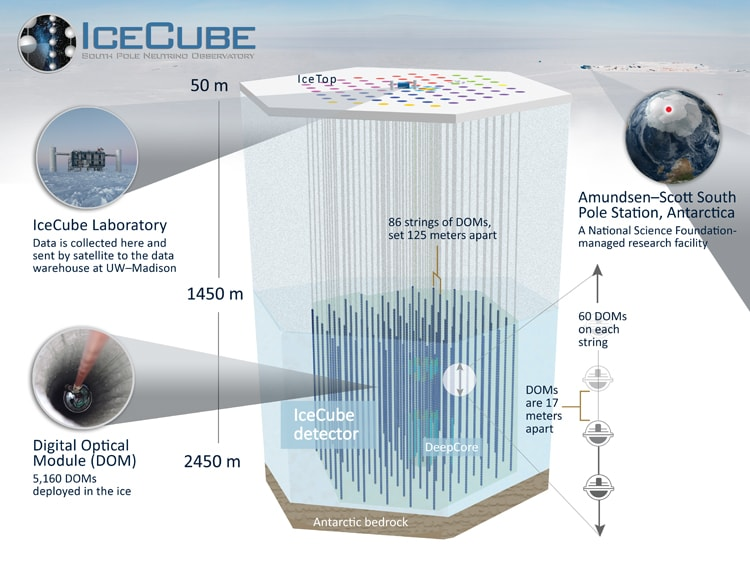
\includegraphics[width=12cm,keepaspectratio]{icecube_detector_schematic.jpeg}
  \caption{Schematic of the IceCube Experiment\cite{IceCube}.}
  \label{fig:IceCube}
\end{figure}

Consisting of the In-Ice Array~\cite{In-Ice}, IceTop~\cite{IceTop} and DeepCore~\cite{DeepCore}, the IceCube experiment is used to study neutrinos and muons. It is located at the Amundsen-Scott South Pole Station near the geographical south pople. The experiment consists of 5160 digital optical modules (DOMs) on 86 strings located $\SIrange{1450}{2450}{\metre}$ under the surface as seen in \autoref{fig:IceCube}. The DOMs are photomultipliers (PMTs) in a vacuumised sphere of glass. These are used to detect the Cherenkov radiation emitted by muons, electrons and tau leptons. Cherenkov radiation is emitted when a relativistic particle travels through a medium with a speed greater than the speed of light in the medium
\begin{equation*}
  c_n = \frac{c_0}{n},
\end{equation*}
where $c_0$ is the speed of light in the vaccum and $n$ is the refractive index of the medium.
The seven strings of DeepCore are as well as their PMTs are spaced more densely, resulting in a lower energy threshold of $\SI{10}{\giga\electronvolt}$ in contrast to a $\SI{100}{\giga\electronvolt}$ energy threshold of the rest of the In-Ice Arry. With the IceTop experiment located at the surface of the south pole air showers are studied. It also functions as a veto for the In-Ice Array.
Neutrinos are measured indirectly via the charged (CC) and neutral currents (NC)
\begin{align*}
&&  \nu_l(\bar{\nu}_l) + A \to l^{\pm} + X && \mathrm{(CC)}\\
&&  \nu_l(\bar{\nu}_l) + A \to \nu_l + X && \mathrm{(NC)}
\end{align*}
where $A$ is a particle the neutrino interacts with and $X$ is a resulting particle shower. Since electrons are highly ionising, they quickly deposit all their energy resulting in a sphere of Cherenkov radiation. The same can be observed for tau leptons because of their short lifetime. Therefore it cannot be distinguished between electron and tau neutrinos, except for the energy of a tau neutrino exceeding $\SI{1}{\peta\electronvolt}$ since then the cascade of the CC interaction and that of the tau lepton decay are spatially separated.
The signature of NC interactions of all lepton flavors induced by the hadron shower is also similar to that of electrons in the CC channel.
Cherenkov radiation emitted by muons is too weak to be detected, but a muon produces $e^+ e^-$ pairs along its way emitting detectable Cherenkov radiation. This results in a cone-like signature for muons.\\

For rejection of atmospheric muons, so called \textit{starting events} are used. Here the outer layers of the detector are used as a veto leading to a smaller effective detector volume, where all neutrino flavors contribute in the same way, meaning that a majority of events are NC processes and CC electron and tau neutrino interactions. These have good energy resolution, but lack a good angle resolution.

Muon tracks have a worse energy resolution, but a higher angle resolution and depending on their energy a higher range allowing to use the earth as shielding, because only muons from neutrino interactions can come from below the detector. To reject atmospheric muons, a cut on the zenith angle can be performed also leading to an enhanced detector volume since also muons from neutrino interactions outisde the detector can be considered. Assuming a perfect reconstruction algorithm, that cut would reject all atmospheric muons. While this is not the case, the cut on the zenith angle still enhances the signal to background ratio from $1 : 10^6$ to $1 : 10^3$. To further improve background rejection machine learning algorithms can be utilised, which is the aim of this analysis.

\section{Multivariate Selection and Machine Learning}

\section{Analysis}\label{sec:Analysis}

\subsection{Data Preparation}

The data used consists of a dataset containing signals generated in a Monte-Carlo simulation and one dataset containing 
background signals also generated in a Monte-Carlo simulation. \\
As the initial step of the analysis the data is prepared.
First all Monte-Carlo truths, event identification numbers and weights are removed so that only the simulated measurements and
event-labels which will later be used for supervised learning are left. In the next step all simulated measurement with missing or
infinite values are removed from the data. Furthermore all columns that contain te same value in every line are deleted.
Finally in both the simulated signal- and backgrounddata attributes which are not contained in the other are removed und
both datasets are combined to one. \\
Finally the data is split in a test- and training-dataset while $80 \, \%$ of the data is used for training and $20 \,\%$
for testing.

\subsection{Forward Selection}

In the next step of the analysis the number of features is reduced by determining the most important features using
the \texttt{SelectKBest} with \texttt{$f\_classif$} from the \texttt{sklearn} library and removing all other features \cite{scikit-learn}. \\
For this the dataset is sequentially reduced to \\
$N \in \{ 10, \, 20, \, 30, \, 40, \, 40, \, 50, \, 60, \, 70, \, 80, \, 90, \, 100 \}$
features and for each number of features the jaccard index is determined for the Naive-Bayes Classifier \texttt{GaussianNB} \cite{scikit-learn}.
In the end the number of features that yields the highest jaccard index is selected for the analysis.
In the run used for the analysis the best jaccard index was archieved for $50$ features. \\
The best $50$ features are determined using \texttt{SelectKBest} and all other features are removed from the data.

\subsection{Training the Classifiers}

For the seperation of the singal data from the background data the classifiers \\ 
\texttt{RandomForestClassifier}, \texttt{KNeighborsClassifier}
and \texttt{GaussianNB} from \texttt{sklearn} are used. in the case of \texttt{RandomForestClassifier} and  \texttt{KNeighborsClassifier}
the optimal number of trees and neighbours is determined analogously to the number of attributes by trying different values and choosing
the value with the largest jaccard index. The optimal values are $N_\text{trees} = 80$ and $N_\text{neighbours} = 50$ \cite{scikit-learn}.\\
All classifiers are trained on the training data and the jaccard index, purity and efficiency are determined by cross validation using 
the method \texttt{cross\_val\_score} \cite{scikit-learn}.
The values are listed in table \ref{tab:results}. \\
Finally a receiver operating characteristic is generated utilising the function \texttt{roc\_curve} and pictured in figure \ref{fig:ROC} \cite{scikit-learn}.

\begin{figure}[tb]
  \centering
  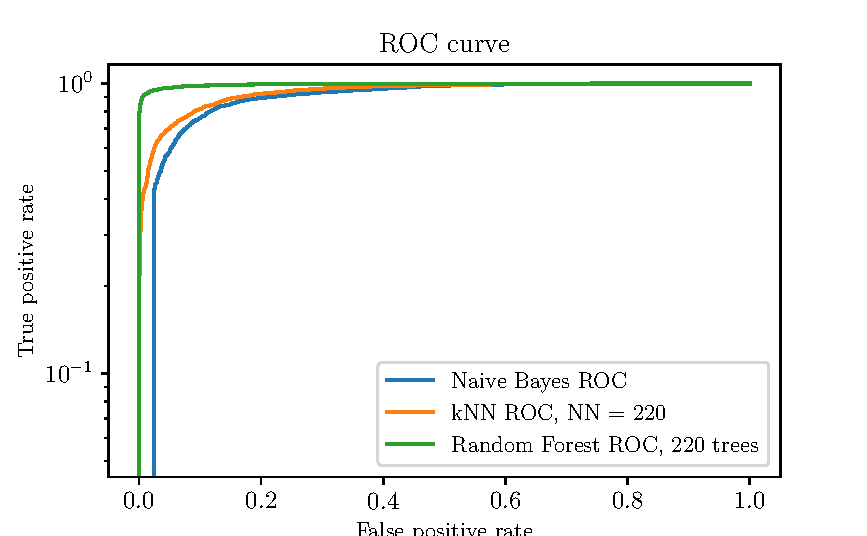
\includegraphics[width=12cm,keepaspectratio]{plots/ROC.pdf}
  \caption{Determined ROC curves for the used classifiers.}
  \label{fig:ROC}
\end{figure}

\begin{table}
  \centering
  \begin{tabular}{c | c c c}
    \toprule
    \text{Classifier} & \text{Efficiency} & \text{Purity} & \text{Jaccard index} \\
    \midrule
    \text{RandomForest} & $\num{0.9525 \pm 0.0085}$ & $\num{0.9651 \pm 0.0829}$ & $\num{0.9187 \pm 0.0757}$ \\
    \text{KNeighborsClassifier} & $\num{0.8540 \pm 0.0215}$ & $\num{0.7661 \pm 0.0621}$ & $\num{0.6769 \pm 0.0407}$ \\
    \text{Naive-Bayes} & $\num{0.7970 \pm 0.0528}$ & $\num{0.7980 \pm 0.0662}$ & $\num{0.6618 \pm 0.0212}$ \\
    \bottomrule
  \end{tabular}
  \caption{Efficiency, purity and Jaccard index of the three classifiers applied to the data set with error estimated by cross validation \cite{scikit-learn}.}
  \label{tab:results}
\end{table}

\section{Diskussion}\label{sec:Durchführung}


\newpage
\nocite{*}
\printbibliography
\appendix
\section{Anhang}
\label{sec:anhang}

\end{document}
